\documentclass{article}
\usepackage[utf8]{inputenc}
\usepackage{amsmath}
\usepackage{float}
\usepackage{listings}
\usepackage[pdftex]{graphicx}
\usepackage{amssymb}
\usepackage{subcaption}
\usepackage{cancel}
\usepackage{float}

\DeclareMathOperator{\sech}{sech}
%---------------------------------------------------------
\author{Pratik Aghor}
\title{HW $\# 2$: Stokes Flow (Flow at Low $Re$)}
\date{\today}  % Toggle commenting to test

\begin{document}

\maketitle
%--------------------------------------------------------
\section{Q $1$: A squirming sheet at zero $Re$: }
%------------------------------------------------
We consider an infinitely-long extensible sheet at $y = 0$ in a viscous fluid. $(x_{s}, y_{s}$ denote the co-ordinates of any particle on the sheet. 
\begin{equation}\label{eq:squriming_sheet}
 x_{s} = x_{0} + a \sin{(kx_{0} - \omega t)}, y_{s} = 0,
\end{equation}
with $x_{0}$ being the time averaged position of any given particle on the sheet and $ak = \epsilon \ll 1$.

In order to find the induced flow, we resort to the stream-function formulation of the Stokes equations. In addition, we impose no-normal flow and no-slip at the surface of the sheet and demand that $u, v$, the $x-$ and $y-$ induced velocities remain bounded. The dimensional governing equation and boundary conditions (BCs) then become:

\begin{align}\label{eq:dim_gov_eqn_bcs}
 \begin{split}
  \left[\frac{\partial^{2}}{\partial x^{2}} + \frac{\partial^{2}}{\partial y^{2}}\right]^{2} \psi &= 0, \\
  \frac{\partial \psi}{\partial x }\bigg|_{x_{s}, 0} & = 0, \\
  \frac{\partial \psi}{\partial y }\bigg|_{x_{s}, 0} &= \frac{dx_{s}}{dt} = - a\omega \cos{(kx_{0} - \omega t)},\\
  \textrm{finally, } \psi & \textrm{ cannot grow more than linear (in x, y) away from the sheet}.
 \end{split}
\end{align}
The condition at infinity ensures that $u, v$ remain bounded at infinity, since $u = \psi_{y}, v = -\psi_{x}$.

We non-dimensionalize the problem by choosing $1/k$ to be the length scale. We choose $a\omega$ to be the velocity scale, inspired by the boundary conditions. 

\begin{equation}\label{eq:squriming_sheet_scalings}
 \tilde{x} = kx, \tilde{y} = ky, \tilde{t} = \omega t, \tilde{u} =  u/(a\omega), \tilde{v} =  v/(a\omega), \tilde{\psi} = \frac{a\omega}{k}\psi. 
\end{equation}

With these scalings, we write the non-dimensional form of Eqns.(\ref{eq:squriming_sheet}) as follows: (dropping tildes):

\begin{align}\label{eq:dimless_gov_eqn_bcs}
 \begin{split}
  x_{s} = x_{0} + \epsilon \sin{(x_{0} - t)},& y_{s} = 0,\\
  \left[\frac{\partial^{2}}{\partial x^{2}} + \frac{\partial^{2}}{\partial y^{2}}\right]^{2} \psi &= 0, \\
  \frac{\partial \psi}{\partial x }\bigg|_{x_{s}, 0} & = 0, \\
  \frac{\partial \psi}{\partial y }\bigg|_{x_{s}, 0} &= -  \cos{(x_{0} - t)},\\
  \textrm{finally, } \psi & \textrm{ cannot grow more than linear (in x, y) away from the sheet}.
 \end{split}
\end{align}

Taylor expanding BCs, around $(x_{0}, 0)$, we obtain:

\begin{align}\label{eq:taylor_exp_bcs}
\begin{split}
 \frac{\partial \psi}{\partial x }\bigg|_{x_{s}, 0} & =  \frac{\partial \psi}{\partial x }\bigg|_{x_{0}, 0} + [\epsilon \sin{(x_{0} - t)}] \frac{\partial^{2} \psi}{\partial x^{2} }\bigg|_{x_{0}, 0}+ O(\epsilon^{2}) = 0.\\
 \frac{\partial \psi}{\partial y }\bigg|_{x_{s}, 0} & = \frac{\partial \psi}{\partial y }\bigg|_{x_{0}, 0} + [\epsilon \sin{(x_{0} - t)} ]\frac{\partial^{2} \psi}{\partial x \partial y }\bigg|_{x_{0}, 0}+ O(\epsilon^{2}) = -  \cos{(x_{0} - t)}.\\
\end{split}
\end{align}

Now, posing a regular perturbation ansatz for $\psi$

\begin{equation}\label{eq:reg_perturb}
 \psi \sim \psi_{0} + \epsilon \psi_{1} + ...,
\end{equation}

and substituting into the dimensionless governing equations and BCs, collecting terms at different orders of $\epsilon$, we get, at $O(1)$:

\begin{align}\label{eq:psi0_eqn}
 \begin{split}
  \left[\frac{\partial^{2}}{\partial x^{2}} + \frac{\partial^{2}}{\partial y^{2}}\right]^{2} \psi_{0} &= 0,\\
 \frac{\partial \psi_{0}}{\partial x }\bigg|_{x_{0}, 0} & = 0\\
 \frac{\partial \psi_{0}}{\partial y }\bigg|_{x_{0}, 0} & = -  \cos{(x_{0} - t)}.
 \end{split}
\end{align}

Guess $\psi_{0} = F(y)\cos{(x-t)}$. Substituting in Eqn.(\ref{eq:psi0_eqn}),

\begin{equation}\label{eqn:F}
 F'''' - 2F'' + F = 0
\end{equation}
where primes denote differentiation wrt argument, here, $y$. 
Linear, constant coefficient, homogeneous ODE, $\Rightarrow F = c e^{\lambda y}$, giving $\lambda^{4} - 2\lambda^{2} + 1 = 0$. This yields $\lambda = \pm 1, \pm 1$. We discard the positive roots owing to the boundedness of velocity fields at infinity, therefore

\begin{equation}\label{eq:F_form}
 \psi_{0} = (A+By) e^{-y}\cos{(x-t)}
\end{equation}
Applying boundary conditions, we get

\begin{align}
 \begin{split}
  &\frac{\partial \psi_{0}}{\partial x }\bigg|_{x_{0}, 0}  = 0\\
  &\Rightarrow (A+By) e^{-y}\sin{(x-t)} \bigg|_{(x_{0}, 0)} = 0 \\
  &\Rightarrow \boxed{A=0}.\\
  &\frac{\partial \psi_{0}}{\partial y }\bigg|_{x_{0}, 0} = -  \cos{(x_{0} - t)}\\
  &Be^{-y}\cos{(x-t)} - Bye^{-y}\cos{(x-t)}\bigg|_{x_{0}, 0} = -  \cos{(x_{0} - t)}\\
  &\Rightarrow \boxed{B=-1}.\\
  & \boxed{\psi_{0} = -y e^{-y}\cos{(x-t)}}
 \end{split}
\end{align}

Going to $O(\epsilon)$, we obtain:
\begin{align}\label{eq:psi1_eqn}
 \begin{split}
  \left[\frac{\partial^{2}}{\partial x^{2}} + \frac{\partial^{2}}{\partial y^{2}}\right]^{2} \psi_{1} &= 0.
 \end{split}
\end{align}
The boundary conditions become:
\begin{align}\label{eq:psi1_x}
 \begin{split}
 &  \frac{\partial \psi_{1}}{\partial x }\bigg|_{x_{0}, 0} + \sin{(x_{0}-t)} \frac{\partial^{2} \psi_{0}}{\partial x^{2}}\bigg|_{x_{0}, 0}= 0\\
 %
 &  \frac{\partial \psi_{1}}{\partial x }\bigg|_{x_{0}, 0} + \sin{(x_{0}-t)} \bigg[\cos{(x_{0}-t)}(-\cancelto{0}{y}e^{-y}) \bigg] = 0\\
 & \boxed{\frac{\partial \psi_{1}}{\partial x }\bigg|_{x_{0}, 0} = 0}.
 \end{split}
\end{align}

\begin{align}\label{eq:psi1_y}
 \begin{split}
 &  \frac{\partial \psi_{1}}{\partial y }\bigg|_{x_{0}, 0} + \sin{(x_{0}-t)} \frac{\partial^{2} \psi_{0}}{\partial x \partial y}\bigg|_{x_{0}, 0}= 0\\
 %
 &  \frac{\partial \psi_{1}}{\partial y }\bigg|_{x_{0}, 0} + \sin{(x_{0}-t)} \bigg[(\cancelto{0}{y}-1)\cancelto{1}{e^{-y}})(-\sin{(x_{0}-t)})\bigg] = 0\\
 & \boxed{\frac{\partial \psi_{1}}{\partial y }\bigg|_{x_{0}, 0} = -\sin^{2}{(x_{0}-t)} = \frac{-1 + \cos{2(x_{0}-t)} }{2}}.
 \end{split}
\end{align}

There is a $-1/2$ factor and $\cos{2(x_{0}-t)} $ factor in the boundary condition, so we guess 

$\boxed{\psi_{1} = f(y) \cos{2(x_{0}-t)} + g(y)}$. Substituting in the Eqn. (\ref{eq:psi1_eqn}), 

\begin{align}
 \begin{split}
  & 16f - 8f'' + f'''' = 0\\
  & g'''' = 0
 \end{split}
\end{align}
Integrating the $g$ equation first, we get 
$g(y) = A_{0} + A_{1}y + A_{2}y^{2} + A_{3}y^{3}$. We put $A_{2} = A_{3} = 0$, owing to boundedness of velocity fields at infinity. Hence, $\boxed{g(y) = A_{0} + A_{1}y}$.

Now, solving the $f$ equation, $f = ce^{\lambda y}$ gives, $\lambda^{4} - 8 \lambda^{2} + 16 = 0$, yielding $\lambda = \pm 2, \pm 2$. Again, we reject positive roots owing to boundedness of velocity fields at infinity. $\boxed{f = (C+Dy)e^{-2y}}$.
Combining $\boxed{\psi_{1}  = A_{0} + A_{1}y + (C+Dy)e^{-2y} \cos{2(x_{0}-t)} }$.
Applying boundary conditions, 
\begin{align}
 \begin{split}
  &\frac{\partial \psi_{1}}{\partial y }\bigg|_{x_{0}, 0} = A_{1} - 2C e^{-2y} \cos{2(x_{0}-t)} + e^{-2y} \cos{2(x_{0}-t)} + D\cancelto{0}{y}...|_{x_{0}, 0} = \frac{-1 + \cos{2(x_{0}-t)} }{2}\\
  & A_{1} + (-2C+D)\cos{2(x_{0}-t)} = \frac{-1 + \cos{2(x_{0}-t)} }{2}.\\
  & \boxed{A_{1} = \frac{1}{2}}, \boxed{D-2C =\frac{1}{2}}.
 \end{split}
\end{align}

\begin{align}
 \begin{split}
  &\frac{\partial \psi_{1}}{\partial x }\bigg|_{x_{0}, 0} = 0\\
  & C \sin{(x_{0} - t)} = 0\\
  & \boxed{C = 0}
 \end{split}
\end{align}
Implying $\boxed{D = 1/2}$. Without loss of generality we substitute $A_{0}=0$ (as we are interested in the gradients of $\psi$, not $\psi$ itself).

$\boxed{\psi_{1} = \frac{y}{2}e^{-2y}\cos{2(x-t)} - \frac{y}{2} }.$
$$u = \frac{\partial \psi}{\partial y} = (y-1)e^{-y} \cos{(x-t)} + \epsilon\left[ \frac{1}{2}e^{-2y} \cos{2(x-t)} - y e^{-2y}\cos{2(x-t)}\right] - \frac{\epsilon}{2}.$$

At infinity, away from the sheet, we obtain a steady streaming flow:
$\boxed{U = -\epsilon/2}$. In dimensional terms, $\boxed{U = -2\pi^{2}\left(\frac{a}{\lambda}\right)^{2}{c}}$, where $\lambda = \frac{2\pi}{k}$ is the wavelength and $c = \frac{\omega}{k}$ is the phase speed. This induced flow is in the opposite direction as that obtained from an undulating sheet (\cite{acheson1991elementary}). 

%--------------------------------------------------------
\section{Q $2$: Drag on a sphere in Stokes flow: }
%------------------------------------------------
We derived the Stokes streamfunction for a Stokes flow past a sphere in class:
\begin{equation}\label{eq:stokes_streamfn}
 \psi(r, \theta) = \frac{1}{4}\bigg(2r^{2}-3r+\frac{1}{r}\bigg)\sin^{2}{\theta}
\end{equation}
Remember the standard $z-$ direction is $x$-direction in our case, in the sense that the polar angle $\theta$ is measured from the $x$- axis. 

The radial and polar velocities are then given by
\begin{align}\label{eq:velo_fields}
 \begin{split}
  u_{r} & = \frac{1}{r^{2}\sin{\theta}}\frac{\partial \psi}{\partial \theta} = \left( 1 - \frac{3}{2r} + \frac{1}{2r^{3}}\right)\cos{\theta}\\
  u_{\theta} &= -\frac{1}{r\sin{\theta}}\frac{\partial \psi}{\partial r} = -\left(1 - \frac{1}{4r^{3}} -\frac{3}{4r} \right)\sin{\theta}
 \end{split}
\end{align}

Integrating the $r$-momentum equation, we find the pressure distribution in the domain:

\begin{align}\label{eq:r_mom}
 \begin{split}
  \nabla p &= \nabla^{2} \boldsymbol{u}\\
  &= \nabla^{2} \boldsymbol{u} - \nabla(\nabla.\boldsymbol{u}) \textrm{ ...} \because \nabla.\boldsymbol{u} = 0\\
  &= -\nabla \times (\nabla \times \boldsymbol{u})\\
  \frac{\partial p}{\partial r} &= -[\nabla \times (\nabla \times \boldsymbol{u})]_{r}\\
  &= -\left[\nabla \times \left(\frac{1}{r} \frac{\partial (r u_{\theta})}{\partial r} - \frac{1}{r}\frac{\partial u_{r}}{\partial \theta}\right) \right]_{r}\\
  &= -\left[\nabla \times \left(\frac{-3\sin{\theta}}{2r^{2}} \hat{e}_{\phi}\right)\right]_{r} \\
  &= \frac{1}{r^{2}\sin{\theta}} \left[\frac{\partial }{\partial \theta}\left(\cancel{r} \sin{\theta} \cdot \frac{3\sin{\theta}}{2r^{\cancel{2} }}  \right) \right]\\
  & = \frac{3\cos{\theta}}{r^{3}}.
 \end{split} 
\end{align}

Integrating from $r$ to $\infty$, we obtain
\begin{align}\label{eq:get_p}
 \begin{split}
  &\int_{r}^{\infty}\frac{\partial p}{\partial r} dr  = \int_{r}^{\infty}\frac{3\cos{\theta}}{r^{3}} dr\\
  & p_{\infty} - p = \frac{3}{2}\frac{\cos{\theta}}{r^{2}}\\
  & \boxed{p = p_{\infty} - \frac{3}{2}\frac{\cos{\theta}}{r^{2}} }.
 \end{split}
\end{align}

We first obtain the stress vector $\tau$ in terms of the stress tensor $\mathcal{T}$. We know, $\tau_{i} = \mathcal{T}_{ij} n_{j}$. For evaluation at the surface of the sphere $r=1$, $n_{j} = \hat{e}_{r} = [1, 0, 0]^{T}$ in spherical polar co-ordinates. We evaluate $\tau_{i}$'s at the surface of the sphere, because we are interested in the drag on the sphere.

\begin{align}\label{eq:stress_vec}
 \begin{split}
  \tau_{r} & = \mathcal{T}_{rr} = [-p + 2 e_{rr}]|_{r=1} \\
  &=  -p_{\infty} + \frac{3}{2}\cos{\theta} \textrm{ ...} \because e_{rr}|_{r=1} = \frac{\partial u_{r}}{\partial r}\bigg|_{r=1} = 0\\
  \tau_{\theta} &= \mathcal{T}_{\theta r} = r \frac{\partial }{\partial r}\left(\frac{u_{\theta}}{r} \right) + \frac{1}{r}\frac{\partial u_{r}}{\partial \theta}\\
  &= -\frac{3}{2}\sin{\theta}\\
  \tau_{\theta} &= \mathcal{T}_{\phi r} = 0.
 \end{split}
\end{align}
To calculate the $x-$component of the stress vector, with a bit of geometry, we can get
\begin{align}
 \begin{split}
  \tau_{x} &= \tau_{r}\cos{\theta} - \tau_{\theta}\sin{\theta}\\
  &=  -p_{\infty} \cos{\theta} + \frac{3}{2}.
 \end{split}
\end{align}
 
The drag on the surface of the sphere ($r=1$) then is given by
\begin{align}\label{eq:dimless_drag}
 \begin{split}
  D &= \int_{0}^{2\pi} \int_{0}^{\pi} \tau_{x} \sin{\theta} d\theta d\phi\\
  &= \cancelto{0}{ \bigg[\int_{0}^{2\pi} \int_{0}^{\pi} -p_{\infty} \cos{\theta} \sin{\theta} d\theta d\phi } \bigg]+ \frac{3}{2} (4 \pi) \\
  &= 6\pi.
 \end{split}
\end{align}

In dimensional terms, we obtain the famous Stokes drag formula $\boxed{D = 6\pi \mu U a}$, where $a$ is the radius of the sphere, moving with velocity $U$ and $\mu$ is the dynamic viscosity. The drag coefficient $C_{D}$ can then be written as 
\begin{equation}\label{eq:cd}
 C_{D} = \frac{D}{\rho U^{2}a^{2}} = \frac{6\pi \mu U a}{ \rho U^{2} a^{2}} = \frac{6\pi}{\frac{\rho U (a)}{\mu}} = \frac{6\pi}{Re}
\end{equation}
where $Re =\frac{\rho U (a)}{\mu}$ is the Reynolds number based on the radius of the sphere.  
%--------------------------------------------------------
\subsection*{Oseen's Improvement }
%------------------------------------------------
The dimensionless Oseen's equation in the frame of reference of the moving sphere (so the sphere is at rest in this frame) are given by:
\begin{align}\label{eq:oseen}
 \begin{split}
  Re \frac{\partial \boldsymbol{u}}{\partial x} &= -\nabla p + \nabla^{2} \boldsymbol{u},\\
 \nabla \cdot \boldsymbol{u} &= 0.
 \end{split}
\end{align}

Taking the curl of Eqn.(\ref{eq:oseen}), and noting that $\nabla \times \nabla p = 0$ identically, we obtain the vorticity form of Oseen's equations.
\begin{align}\label{eq:oseen_vort}
 \begin{split}
  Re \frac{\partial \boldsymbol{\omega}}{\partial x} &= \nabla^{2} \boldsymbol{\omega}\\
  Re \left(\frac{1}{\cos{\theta}}\frac{\partial \boldsymbol{\omega}}{\partial r} - \frac{1}{r\sin{\theta}} \frac{\partial \boldsymbol{\omega}}{\partial \theta} \right)&= \nabla^{2} \boldsymbol{\omega} \textrm{ ...}\because x = r\cos{\theta}
 \end{split}
\end{align}

In the axisymmetric case, substituting $u_{r}, u_{\theta}$ from Eqn.(\ref{eq:velo_fields}),
\begin{align}\label{eq:omega}
 \begin{split}
  \boldsymbol{\omega} &= \left(\frac{1}{r} \frac{\partial (r u_{\theta})}{\partial r} - \frac{1}{r}\frac{\partial u_{r}}{\partial \theta}\right) \hat{e}_{\phi} \\
  &= \left(\frac{1}{r} \frac{\partial }{\partial r} \left[\cancel{r} \left(  -\frac{1}{\cancel{r}\sin{\theta}}\frac{\partial \psi}{\partial r} \right) \right]- \frac{1}{r}\frac{\partial }{\partial \theta}\left[ \frac{1}{r^{2}\sin{\theta}}\frac{\partial \psi}{\partial \theta} \right]\right) \hat{e}_{\phi}\\
  & = \left(-\frac{1}{r\sin{\theta}}\frac{\partial^{2} \psi}{\partial r^{2}} - \frac{1}{r^{3}}\left[-\frac{\cot{\theta}}{\sin{\theta}} \frac{\partial \psi}{\partial \theta} + \frac{1}{\sin{\theta}} \frac{\partial^{2}\psi}{\partial\theta^{2}} \right]\right) \hat{e}_{\phi}\\
  & = -\frac{1}{r\sin{\theta}} D^{2} \psi
 \end{split}
\end{align}
where $D^{2}$ is given by

\begin{equation}\label{eq:Dsq}
 D^{2} = \left[\frac{\partial^{2} }{\partial r^{2}} + \frac{1}{r^{2}}\frac{\partial^{2}}{\partial \theta^{2}} - \frac{\cot{\theta}}{r^{2}}\frac{\partial}{\partial \theta} \right]\textrm{ ...(NOTE:} D^{2}\neq\nabla^{2}).
\end{equation}

Substituing Eqn. (\ref{eq:omega}) in Eqn. (\ref{eq:oseen_vort}), we get

\begin{equation}\label{eq:biharmonic_oseen_1}
 \left(\frac{1}{Re}D^{2} - \cos{\theta}\frac{\partial }{\partial r} + \frac{\sin \theta}{r}\frac{\partial }{\partial \theta}\right)D^{2}\psi = 0.
\end{equation}

Writing $\cos{\theta} = c$ we get
\begin{align}\label{eq:biharmonic_oseen_2}
 \begin{split}
  \left(\frac{1}{Re}D^{2} - \cos{\theta}\frac{\partial }{\partial r} + \frac{\sin \theta}{r}\frac{\partial }{\partial \theta}\right)D^{2}\psi &= 0.\\
  %
  \left(\frac{1}{Re}D^{2} - c \frac{\partial }{\partial r} + \frac{(1-c^{2})^{1/2}}{r}\frac{\partial }{\partial \theta}\right)D^{2}\psi &= 0.\\
  %
  \left(\frac{1}{Re}D^{2} - c \frac{\partial }{\partial r} + \frac{(1-c^{2})^{1/2}}{r}\cancelto{-(1-c^{2})^{1/2}}{\frac{dc}{d\theta}}\frac{\partial }{\partial c}\right)D^{2}\psi &= 0.\\
  %
  \left(\frac{1}{Re}D^{2} - c \frac{\partial }{\partial r} - \frac{(1-c^{2})}{r}\frac{\partial }{\partial c}\right)D^{2}\psi &= 0.\\
 \end{split}
\end{align}

We are asked to verify by direct substitution that $\psi(r, \theta; Re) = (1+c)[1 - e^{-\frac{1}{2} Re r(1-c)}]$ satisfies Eqn. (\ref{eq:biharmonic_oseen_2}).

First, we convert the $D^{2}(r, \theta)$ into $D^{2}(r, c)$. 

Using chain rule, we have $\frac{\partial }{\partial \theta} = \frac{\partial c}{\partial \theta}\frac{\partial }{\partial c} = -(1-c^{2})^{1/2}\frac{\partial }{\partial c}$. Similarly, applying $\frac{\partial }{\partial \theta}$ one more time, we obtain:

\begin{align}
 \begin{split}
 \frac{\partial^{2} }{\partial \theta^{2}} &= \cancelto{-(1-c^{2})^{1/2}}{\frac{\partial c}{\partial \theta}} \frac{\partial }{\partial c} \left(-(1-c^{2})^{1/2}\frac{\partial }{\partial c} \right)\\
 &= (1-c^{2})^{1/2}\left( (1-c^{2})^{1/2}\frac{\partial^{2} }{\partial c^{2}} - \frac{c}{(1-c^{2})^{1/2}}\frac{\partial}{\partial c} \right)\\
 &=(1-c^{2})\frac{\partial^{2} }{\partial c^{2}} - c\frac{\partial}{\partial c}
 \end{split}
\end{align}

\begin{align}\label{eq:Dsq_2}
 \begin{split}
  & D^{2} = \left[\frac{\partial^{2} }{\partial r^{2}} + \frac{1-c^{2}}{r^{2}} \frac{\partial^{2} }{\partial c^{2}} - \cancel{\frac{c}{r^{2}}\frac{\partial}{\partial c} }+ \cancel{\frac{c}{r^{2}}\frac{\partial}{\partial c} }\right]\\
 &\boxed{D^{2} = \left[ \frac{\partial^{2} }{\partial r^{2}} + \frac{1-c^{2}}{r^{2}} \frac{\partial^{2} }{\partial c^{2}}\right] }
 \end{split}
\end{align}

Let us find $D^{2}\psi$ now.
\begin{align}\label{eq:D2psi}
 \begin{split}
  D^{2}\psi &= \left[ \frac{\partial^{2}}{\partial r^{2}}(1+c)[1 - e^{-\frac{1}{2} Re r(1-c)}]  + \frac{1-c^{2}}{r^{2}} \frac{\partial^{2} }{\partial c^{2}}(1+c)[1 - e^{-\frac{1}{2} Re r(1-c)}] \right] \\
  &= \frac{Re^{2}}{4}  (1-c^{2})^{2}e^{-\frac{1}{2} Re r(1-c)} -  \frac{1-c^{2}}{r^{2}}e^{-\frac{1}{2} Re r(1-c)}\left[\frac{1}{4}Re^{2}r^{2} + \frac{cRe r}{2} + 1 \right]
 \end{split}
\end{align}
Substituing Eqn.(\ref{eq:D2psi})into Eqn. (\ref{eq:biharmonic_oseen_2}), I verified that $\psi(r, \theta; Re) = (1+c)[1 - e^{-\frac{1}{2} Re r(1-c)}]$ satisfies Eqn. (\ref{eq:biharmonic_oseen_2}). 
I did not have enough time to verify or type out that the following stream function also satisfies Eqn. (\ref{eq:biharmonic_oseen_2}) and the boundary conditions $\psi = \frac{\partial \psi}{\partial r} = 0 $ on $r = 1$ and $\psi \sim \frac{r^{2}}{2}\sin{\theta}$ as $r\rightarrow \infty$.
\begin{equation}\label{eq:oseen_psi}
 \psi(r, \theta;Re) \sim \left(\frac{r^{2}}{2} + \frac{1}{4r}\right)\sin^{2}{\theta} - \frac{3}{2Re}(1+c)[1 - e^{-\frac{1}{2} Re r(1-c)}]. 
\end{equation}
I did plot it though. As can be seen fro Fig.(\ref{fig:oseen_streamlines}), the flow at $Re=0.1$ is fore-aft symmetric, while the flow at $Re=1$ breaks the fore-aft symmetry.
\begin{figure}[H]
     \centering
     \begin{subfigure}[b]{0.49\textwidth}
         \centering
         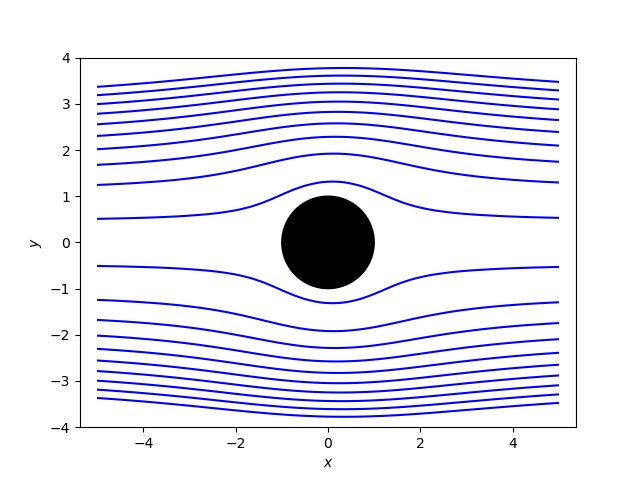
\includegraphics[scale = 0.4]{Figs/oseen_Re_0_1.png}
         \caption{$Re=0.1$}
         \label{fig:Re_0.1}
     \end{subfigure}
     \begin{subfigure}[b]{0.49\textwidth}
         \centering
         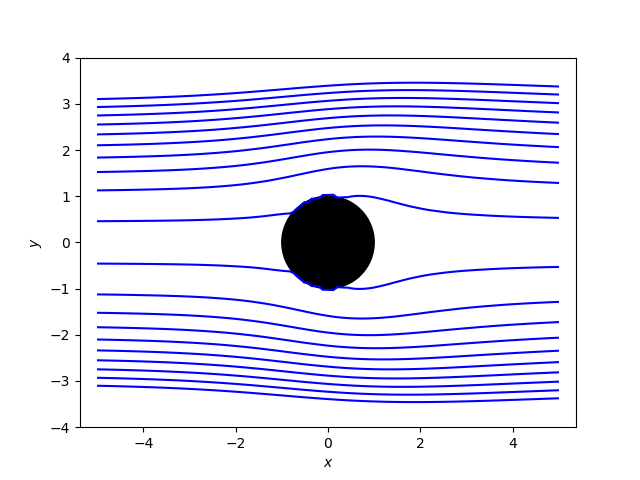
\includegraphics[scale = 0.4]{Figs/oseen_Re_1.png}
         \caption{$Re=1$}
         \label{fig:Re_1}
     \end{subfigure}
     \caption{Flow at $Re=1$ breaks the fore-aft symmetry.}
  \label{fig:oseen_streamlines}
\end{figure}
%--------------------------------------------------------
\section{Q $3$: Superposition of singular solutions of Stokes flow: }
%------------------------------------------------
\subsection*{Velocity field due to a single Stokeslet:}
We derived in class the strema-function $\psi$ due to a Stokeslet of strength $F$ situated at the origin. 
\begin{equation}\label{eq:psi_stokeslet}
 \psi \sim -\frac{3}{4} r \sin^{2}{\theta}
\end{equation}

This gives the induced velocity field to be 
\begin{equation}\label{eq:velo_stokeslet}
 u(r, \theta, \phi) = \frac{F}{8\pi\mu}\left(\frac{2\cos{\theta}}{r}, -\frac{\sin{\theta}}{r}\right)
\end{equation}

We can write this in terms of Cartesian co-ordinates, with 
\begin{equation}\label{eq:velo_stokeslet_2}
 u(x, y) = \frac{F}{8\pi\mu}\left(\frac{2x}{(x^{2}+y^{2})}, -\frac{y}{(x^{2}+y^{2})}\right)
\end{equation}
The unit vectors are still $\hat{e}_{r}$, $\hat{e}_{\theta}$. In order to get to Cartesian co-ordinates, $\hat{e}_{x} = \cos{\theta}\hat{e}_{r} - \sin{\theta}\hat{e}_{\theta}$, $\hat{e}_{y} = \sin{\theta}\hat{e}_{r} + \cos{\theta}\hat{e}_{\theta}$. Moreover, we have $\tan{\theta} = y/x$, giving $\cos{\theta} = x/(x^{2}+r^{2})^{1/2}$ and $\sin{\theta} = y/(x^{2}+r^{2})^{1/2}$, yielding

\begin{equation}\label{eq:u_stokeslet_cartesian}
 \boldsymbol{u}(x, y) = \frac{F}{8\pi\mu}\left(\frac{2x^{2}+y^{2}}{(x^{2}+y^{2})^{3/2}} \hat{e}_{x} + \frac{xy}{(x^{2}+y^{2})^{3/2}} \hat{e}_{y} \right)
\end{equation}

Similarly, the stremfunction $\psi(x, y) = -\frac{3}{4} \frac{y^{2}}{(x^{2}+y^{2})^{1/2}}$. I plotted this using python:
\begin{figure}[H]
    \centering
    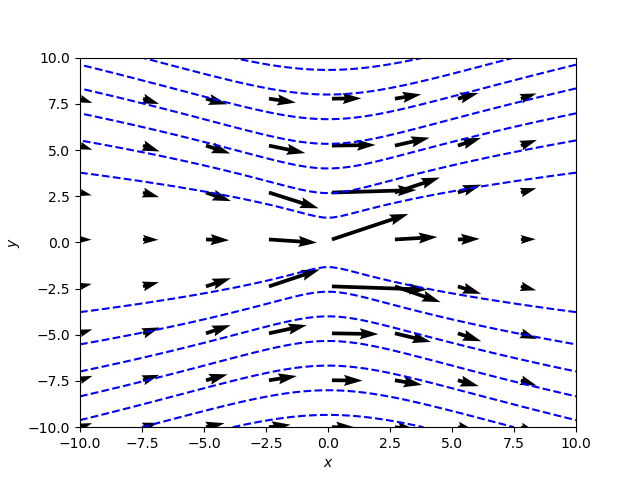
\includegraphics[scale = 0.8]{Figs/stokeslet.png}
    \caption{Flow induced due to a single Stokeslet. Near (0,0) we get singular behavior. The dashed blue lines represent contours of the stream function $\psi$.}
    \label{fig:stokeslet}
\end{figure}

%
\subsection*{Finite slender cylinder:}
Consider a finite slender cylinder ($x=-b$ to $x=c$), with radius $a$ ($b, c \gg a$), moving in a direction parallel to its axis. We want to derive an expression for the induced velocity field due to a line of Stokeslets of strength $(fdx, 0, 0)$, distributed along its centerline. 

Without loss of generality, we consider a Stokeslet sitting at $X=0$. The distance $r$ of any point in the domain from the surface of the cylinder is then approximately given by $r^{2} = (x-X)^{2} + y^{2} + z^{2}$. On the surface of the cylinder $y^{2} + z^{2} = a^{2}$, hence, $\boxed{r^{2} = x^{2} + a^{2}}$. 

\begin{equation}\label{eq:du_stokeslet}
 \boldsymbol{du}_{Stokeslet}\bigg|_{X = 0, y^{2}+z^{2} = a^{2}} = \frac{f}{8\pi \mu} \left(\frac{x^{2} + r^{2}}{r^{3}}, \frac{xy}{r^{3}}, \frac{xz}{r^{3}} \right).
\end{equation}

In order to calculate the induced field due to a continuum of Stokeslets, we must integrate

\begin{equation}
 \boldsymbol{u}_{Stokeslet} = \frac{f}{8\pi \mu}\int_{x=-b}^{c}\left(\frac{x^{2} + r^{2}}{r^{3}}, \frac{xy}{r^{3}}, \frac{xz}{r^{3}} \right) = I_{1}\hat{e}_{x} + I_{2}\hat{e}_{y} + I_{3}\hat{e}_{z}.
\end{equation}
Let us focus on the $I_{2}$ and $I_{3}$ integrals first. The integrals will be of the form $\int_{-b}^{c}\frac{x}{r^{3}}dx$. Changing variables to $\chi = x/a$

\begin{equation}
 I_{2, 3} \sim \int_{-b/a \rightarrow -\infty}^{c/a \rightarrow \infty} \frac{x}{r^{3}} dx
\end{equation}

But $\frac{x}{(x^{2}+a^{2})^{3/2}}$ is an odd function of $x$, hence on a symmetric interval, $I_{2}, I_{3}$ will vanish. In this case, they will vanish owing to the `slender-ness' of the cylinder. 

Now, let's focus on the $I_{1}$ integral. 
\begin{align}
 \begin{split}
  I_{1} &\sim \int_{x=-b}^{c} \frac{x^{2} + r^{2}}{r^{3}} dx\\
  &\sim \int_{x=-b}^{c} \frac{x^{2} + x^{2} + a^{2}}{r^{3}} dx\\
  &\sim \int_{x=-b}^{c} \frac{2(x^{2} + a^{2}) - a^{2}}{r^{3}} dx\\
  &\sim 2\int_{x=-b}^{c} \frac{dx}{(x^{2} + a^{2})^{1/2}} - a^{2}\int_{x=-b}^{c} \frac{dx}{(x^{2} + a^{2})^{3/2}}\\
  &\textrm{chaning variables to } \chi = x/a  \textrm{, and noting } b/a, c/a \rightarrow \infty\\
  &\sim 2 \int_{-b/a}^{c/a} \frac{d\chi}{(1+\chi^{2})^{1/2}} - \int_{-b/a}^{c/a} \frac{d\chi}{(1+\chi^{2})^{3/2}}\\
  &\textrm{substituting }\chi = \sinh(\phi)\\
  &\sim 2\left[\sinh^{-1}\left(\frac{c}{a}\right) + \sinh^{-1}\left(\frac{b}{a}\right)\right] - 2\\
  &\sim 2 \ln{\frac{4cb}{a^{2}}} - 2
 \end{split}
\end{align}
Therefore
\begin{equation}\label{eq:u_stokeslet}
 \boldsymbol{u}_{Stokeslet} = \frac{f}{8\pi \mu} \left(2 \ln{\frac{4cb}{a^{2}}} - 2, 0, 0\right)
\end{equation}

This already gives the uniform flow at the surface of a cylinder, so we expect that the doublet contribution would be zero or a constant. Let us calculate the induced velocity due to a source-doublet distribution of to-be-determined strength $(gdx, 0, 0)$. As for the Stokeslet, to obtain the total induced velocity we  integrate the velocity field induced by doublets along the axis of the cylinder. 

\begin{equation}
 \boldsymbol{u}\bigg|_{doublet} = \frac{g}{4\pi}\int_{x=-b}^{c}\left( \frac{1}{r^{3}} - \frac{3x^{2}}{r^{5}}, \frac{-3xy}{r^{5}}, \frac{3xz}{r^{5}}\right)dx=  I_{1d}\hat{e}_{x} + I_{2d}\hat{e}_{y} + I_{3d}\hat{e}_{z}.
\end{equation}
The subscript `d' denotes the contribution due to doublets. As before, the $I_{2d}, I_{3d}$ vanish owing to the `odd-ness' of $x/r^{5}$ in $x$, in the limit $b/a, c/a \rightarrow \infty$. 

Consider 
\begin{align}
 \begin{split}
  I_{1d} &\sim \int_{-b}^{c}\frac{dx}{(x^{2}+a^{2})^{3/2}} - \int_{-b}^{c}\frac{3x^{2}}{(x^{2}+a^{2})^{5/2}} dx\\
  &\textrm{the first part, as above }=\frac{2}{a^{2}}\\
  &\sim \frac{2}{a^{2}} - 3\int_{-b}^{c}\frac{x^{2} + a^{2} - a^{2}}{(x^{2}+a^{2})^{5/2}} dx \\
  &\textrm{ changing variable to } \chi = x/a\\
  &\sim \frac{2}{a^{2}} - \frac{3}{a^{2}}\left(\cancelto{2}{\int_{-\infty}^{\infty} \frac{d\chi}{(1+\chi^{2})^{3/2}} } - \int_{-\infty}^{\infty} \frac{d\chi}{(1+\chi^{2})^{5/2}} \right)\\
  &\textrm{substituting }\chi = \sinh{\phi}\\
  &\sim \frac{2}{a^{2}} - \frac{3}{a^{2}}\left(2 - \int_{-\infty}^{\infty} \sech^{4}{\phi}d\phi\right)\\
  &\sim \frac{2}{a^{2}} - \frac{3}{a^{2}}\left(2 - \frac{1}{3}\left[\left(\frac{\cancel{e^{2\phi} + e^{-2\phi}}}{2} + 2\right) \tanh{\phi} \frac{4}{\cancel{(e^{\phi}+e^{-\phi})^{2}}}\right]_{-\infty}^{\infty}\right)\\
  &\textrm{The cancelled terms above cancel each other in the limit }\pm \infty\\
  &\sim \frac{2}{a^{2}} - \frac{3}{a^{2}}\left(2 - \frac{1}{3}\left[ \frac{1}{2}\right]\cdot(1-(-1))\cdot 4\right)\\
  &\sim \frac{2}{a^{2}} - \frac{3}{a^{2}}\left(2 - \frac{4}{3}\right)\\
  &=0
 \end{split}
\end{align}
As expected, the doublet contribution comes out to be exactly $\boldsymbol{0}$. Hence any finite $g$ would do the job, since the contribution from the doubltes is nil. The total induced velocity field is then 
\begin{equation}\label{eq:u}
 \boldsymbol{u} = \boldsymbol{u}_{Stokeslet} = \frac{f}{8\pi \mu} \left(2 \ln{\frac{4cb}{a^{2}}} - 2, 0, 0\right)
\end{equation}

%------------------------------------------------------
\bibliographystyle{apalike}
%\bibliographystyle{unsrt} % Use for unsorted references  
%\bibliographystyle{plainnat} % use this to have URLs listed in References
%\cleardoublepage
%\bibliography{References/references} % Path to your References.bib file

\bibliography{bib/references} % Path to your References.bib file
 \if@openright\cleardoublepage\else\clearpage\fi
 \cleardoublepage
 \pagestyle{empty}
%--------------------------------------------------------------------
\end{document}
